\chapter{Ordinamento}

\index{ordinamento}

\key{L'ordinamento}
è uno dei problemi classici dell'informatica.
Molti algoritmi efficienti 
al loro interno usano l'ordinamento come
passaggio verso la soluzione del problema,
poichè è spesso più facile processare i dati
se gli elementi sono ordinati. 

Per esempio, il problema "l'array contiene due elementi uguali?",
può essere risolto facilmente usando l'ordinamento.
Se l'array contiene due elementi uguali
e il vettore è ordinato, saranno uno dopo l'altro e 
quindi saranno facili da trovare.
Anche il problema "qual è l'elemento più frequente nell'array"
è facile da risolvere una volta ordinato il vettore.

Esistono molti algoritmi per ordinare un vettore, che
permettono anche di mostrare differenti 
tecniche di progettazione.
I migliori algoritmi di ordinamento di carattere generale
sono di classe $O(n \log n)$ e molti
algoritmi che usano l'ordinamento come passaggio
intermedio hanno anch'essi questo tipo di complessità. 

\section{Il problema dell'ordinamento}

La forma base del problema dell'ordinamento  è la seguente:
\begin{framed}
\noindent
Dato un array contenente $n$ elementi, 
disporre gli elementi in ordine crescente.
\end{framed}
\noindent
Per esempio, l'array
\begin{center}
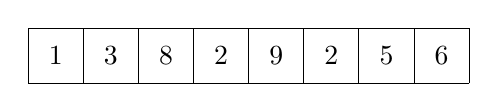
\begin{tikzpicture}[scale=0.7]
\draw (0,0) grid (8,1);
\node at (0.5,0.5) {$1$};
\node at (1.5,0.5) {$3$};
\node at (2.5,0.5) {$8$};
\node at (3.5,0.5) {$2$};
\node at (4.5,0.5) {$9$};
\node at (5.5,0.5) {$2$};
\node at (6.5,0.5) {$5$};
\node at (7.5,0.5) {$6$};
\end{tikzpicture}
\end{center}
dopo l'ordinamento diventerà:
\begin{center}
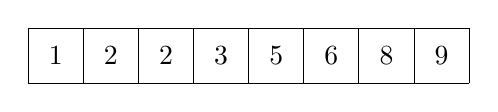
\begin{tikzpicture}[scale=0.7]
\draw (0,0) grid (8,1);
\node at (0.5,0.5) {$1$};
\node at (1.5,0.5) {$2$};
\node at (2.5,0.5) {$2$};
\node at (3.5,0.5) {$3$};
\node at (4.5,0.5) {$5$};
\node at (5.5,0.5) {$6$};
\node at (6.5,0.5) {$8$};
\node at (7.5,0.5) {$9$};
\end{tikzpicture}
\end{center}

\subsubsection{Algoritmi con complessità $O(n^2)$}

\index{bubble sort}

Gli algoritmi più semplici per ordinare un vettore
hanno una complessità di tipo $O(n^2)$.
Solitamente sono corti da scrivere e sono formati da 
due cicli annidati.
Un famoso algoritmo di tipo $O(n^2)$ è il
\key{bubble sort}, dove gli elementi risalgono il vettore
come "bolle" di gas in un liquido in base al proprio valore.
Il bubble sort consiste di $n$ passaggi, in ognuno dei quali
si scorre tutto il vettore. Quando vengono trovati due elementi consecutivi 
che non sono nell'ordine corretto, questi vengono scambiati.
Un'implementazione di questo algoritmo è la seguente:
\begin{lstlisting}
for (int i = 0; i < n; i++) {
    for (int j = 0; j < n-1; j++) {
        if (array[j] > array[j+1]) {
            swap(array[j],array[j+1]);
        }
    }
}
\end{lstlisting}

Dopo il primo passaggio, l'elemento maggiore sarà nella sua posizione
corretta in fondo al vettore e, in generale, dopo $k$ passaggi,
i $k$ elementi più grandi del vettore saranno nella
loro posizione finale.
Quindi dopo $n$ passaggi, tutto il vettore 
risulterà ordinato.

Per esempio, nell'array

\begin{center}
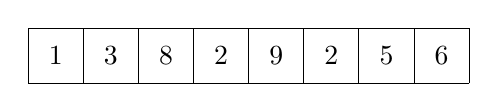
\begin{tikzpicture}[scale=0.7]
\draw (0,0) grid (8,1);

\node at (0.5,0.5) {$1$};
\node at (1.5,0.5) {$3$};
\node at (2.5,0.5) {$8$};
\node at (3.5,0.5) {$2$};
\node at (4.5,0.5) {$9$};
\node at (5.5,0.5) {$2$};
\node at (6.5,0.5) {$5$};
\node at (7.5,0.5) {$6$};
\end{tikzpicture}
\end{center}

\noindent
il primo passaggio scambierà gli elementi nel seguente modo:

\begin{center}
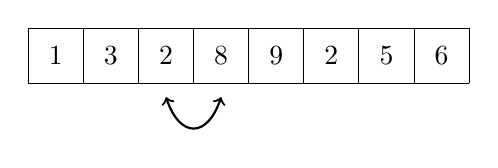
\begin{tikzpicture}[scale=0.7]
\draw (0,0) grid (8,1);
\node at (0.5,0.5) {$1$};
\node at (1.5,0.5) {$3$};
\node at (2.5,0.5) {$2$};
\node at (3.5,0.5) {$8$};
\node at (4.5,0.5) {$9$};
\node at (5.5,0.5) {$2$};
\node at (6.5,0.5) {$5$};
\node at (7.5,0.5) {$6$};

\draw[thick,<->] (3.5,-0.25) .. controls (3.25,-1.00) and (2.75,-1.00) .. (2.5,-0.25);
\end{tikzpicture}
\end{center}

\begin{center}
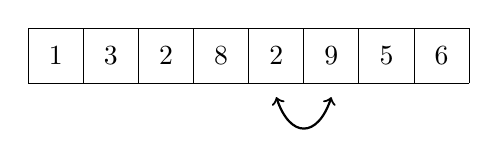
\begin{tikzpicture}[scale=0.7]
\draw (0,0) grid (8,1);
\node at (0.5,0.5) {$1$};
\node at (1.5,0.5) {$3$};
\node at (2.5,0.5) {$2$};
\node at (3.5,0.5) {$8$};
\node at (4.5,0.5) {$2$};
\node at (5.5,0.5) {$9$};
\node at (6.5,0.5) {$5$};
\node at (7.5,0.5) {$6$};

\draw[thick,<->] (5.5,-0.25) .. controls (5.25,-1.00) and (4.75,-1.00) .. (4.5,-0.25);
\end{tikzpicture}
\end{center}

\begin{center}
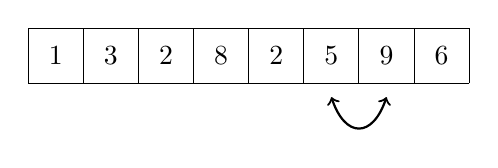
\begin{tikzpicture}[scale=0.7]
\draw (0,0) grid (8,1);
\node at (0.5,0.5) {$1$};
\node at (1.5,0.5) {$3$};
\node at (2.5,0.5) {$2$};
\node at (3.5,0.5) {$8$};
\node at (4.5,0.5) {$2$};
\node at (5.5,0.5) {$5$};
\node at (6.5,0.5) {$9$};
\node at (7.5,0.5) {$6$};

\draw[thick,<->] (6.5,-0.25) .. controls (6.25,-1.00) and (5.75,-1.00) .. (5.5,-0.25);
\end{tikzpicture}
\end{center}

\begin{center}
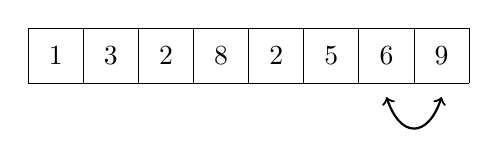
\begin{tikzpicture}[scale=0.7]
\draw (0,0) grid (8,1);
\node at (0.5,0.5) {$1$};
\node at (1.5,0.5) {$3$};
\node at (2.5,0.5) {$2$};
\node at (3.5,0.5) {$8$};
\node at (4.5,0.5) {$2$};
\node at (5.5,0.5) {$5$};
\node at (6.5,0.5) {$6$};
\node at (7.5,0.5) {$9$};

\draw[thick,<->] (7.5,-0.25) .. controls (7.25,-1.00) and (6.75,-1.00) .. (6.5,-0.25);
\end{tikzpicture}
\end{center}

\subsubsection{Inversioni}

\index{inversione}

Il bubble sort è un esempio di algoritmo di ordinamento
che scambia sempre due elementi \emph{consecutivi} nell'array. 
Si può vedere che la complessità di questo algoritmo,
nel caso peggiore, è sempre $O(n^2)$, 
perchè sono richiesti $O(n^2)$ scambi per ordinare l'array. 

Un concetto utile quando si analizzano gli algoritmi di ordinamento
è quello di \key{inversione}: si dice inversione una coppia di elementi 
$(\texttt{array}[a],\texttt{array}[b])$ tale che 
$a<b$ e $\texttt{array}[a]>\texttt{array}[b]$,
cioè quando gli elementi non sono nell'ordine corretto.

Per esempio, l'array

\begin{center}
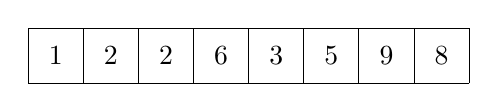
\begin{tikzpicture}[scale=0.7]
\draw (0,0) grid (8,1);
\node at (0.5,0.5) {$1$};
\node at (1.5,0.5) {$2$};
\node at (2.5,0.5) {$2$};
\node at (3.5,0.5) {$6$};
\node at (4.5,0.5) {$3$};
\node at (5.5,0.5) {$5$};
\node at (6.5,0.5) {$9$};
\node at (7.5,0.5) {$8$};
\end{tikzpicture}
\end{center}
ha tre inversioni: $(6,3)$, $(6,5)$ e $(9,8)$.
Il numero di inversioni indica quando
lavoro deve essere fatto per ordinare l'array,
difatti un array è completamente ordinato 
quando non ci sono più inversioni.
D'altra parte, se l'array è ordinato al contrario,
il numero di inversioni è il più grande possibile:

\[1+2+\cdots+(n-1)=\frac{n(n-1)}{2} = O(n^2)\]

Scambiare una coppia di elementi consecutivi che sono
nell'ordine sbagliato, rimuove esattamente un'inversione.
Qundi, se un algoritmo è in grado di scambiare solo
elementi consecutivi, ogni scambio rimuove al massimo
un'inversione, e la complessità dell'algoritmo è di tipo $O(n^2)$

\subsubsection{Algoritmi di tipo $O(n \log n)$}

\index{merge sort}

È possibile ordinare un array in maniera efficiente usando
degli algoritmi che non si limitano allo scambio di elementi
consecutivi, arrivando a una  complessità di tipo $O(n \log n)$.

Uno di questi algoritmi è il \key{merge sort}\footnote{Secondo \cite{knu983},
il merge sort è stato inventato da J. von Neumann nel 1945.}
e per risolvere il problema utilizza la ricorsione.

Il merge sort ordina un sottovettore \texttt{array}$[a \ldots b]$ nel modo seguente:

\begin{enumerate}
\item Se $a=b$ non si fa niente, perchè il sottovettore è già ordinato.
\item Si calcoli la posizione dell'elemento mediano: $k=\lfloor (a+b)/2 \rfloor$.
\item Si ordini ricorsivamente il sottovettore \texttt{array}$[a \ldots k]$.
\item Si ordini ricorsivamente il sottovettore \texttt{array}$[k+1 \ldots b]$.
\item Si fondano (\emph{merge}) i sottovettori ordinati \texttt{array}$[a \ldots k]$ e
\texttt{array}$[k+1 \ldots b]$
in un array ordinato \texttt{array}$[a \ldots b]$.
\end{enumerate}

Il merge sort è un algoritmo efficiente perchè
dimezza la dimensione del sottovettore a ogni passaggio.
Quindi la ricorsione consiste di $O(\log n)$ livelli e 
ogni livello richiede $O(n)$ operazioni.
Fondere i sottovettori \texttt{array}$[a \ldots k]$ e \texttt{array}$[k+1 \ldots b]$
è un'operazione che può essere eseguita in tempo lineare, perchè entrambi sono già ordinati.

Per esempio, si condideri il seguente array:

\begin{center}
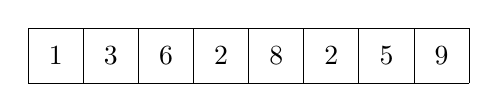
\begin{tikzpicture}[scale=0.7]
\draw (0,0) grid (8,1);
\node at (0.5,0.5) {$1$};
\node at (1.5,0.5) {$3$};
\node at (2.5,0.5) {$6$};
\node at (3.5,0.5) {$2$};
\node at (4.5,0.5) {$8$};
\node at (5.5,0.5) {$2$};
\node at (6.5,0.5) {$5$};
\node at (7.5,0.5) {$9$};
\end{tikzpicture}
\end{center}

L'array verrà suddiviso nei due sottoarray come segue:

\begin{center}
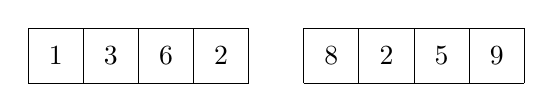
\begin{tikzpicture}[scale=0.7]
\draw (0,0) grid (4,1);
\draw (5,0) grid (9,1);

\node at (0.5,0.5) {$1$};
\node at (1.5,0.5) {$3$};
\node at (2.5,0.5) {$6$};
\node at (3.5,0.5) {$2$};

\node at (5.5,0.5) {$8$};
\node at (6.5,0.5) {$2$};
\node at (7.5,0.5) {$5$};
\node at (8.5,0.5) {$9$};
\end{tikzpicture}
\end{center}

Successivamente i due sottovettori verranno ordinati ricorsivamente:

\begin{center}
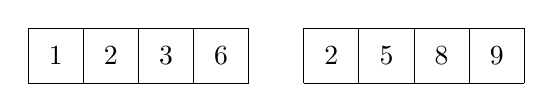
\begin{tikzpicture}[scale=0.7]
\draw (0,0) grid (4,1);
\draw (5,0) grid (9,1);

\node at (0.5,0.5) {$1$};
\node at (1.5,0.5) {$2$};
\node at (2.5,0.5) {$3$};
\node at (3.5,0.5) {$6$};

\node at (5.5,0.5) {$2$};
\node at (6.5,0.5) {$5$};
\node at (7.5,0.5) {$8$};
\node at (8.5,0.5) {$9$};
\end{tikzpicture}
\end{center}

Infine l'algoritmo fonderà i due sottovettori ordinati
e creerà il vettore finale ordinato:

\begin{center}
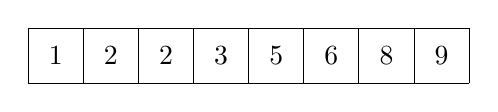
\begin{tikzpicture}[scale=0.7]
\draw (0,0) grid (8,1);
\node at (0.5,0.5) {$1$};
\node at (1.5,0.5) {$2$};
\node at (2.5,0.5) {$2$};
\node at (3.5,0.5) {$3$};
\node at (4.5,0.5) {$5$};
\node at (5.5,0.5) {$6$};
\node at (6.5,0.5) {$8$};
\node at (7.5,0.5) {$9$};
\end{tikzpicture}
\end{center}

\subsubsection{Limite inferiore per il problema dell'ordinamento}

È possibile ordinare un vettore in un tempo 
inferiore a $O(n \log n)$?
Si può verificare che questo \emph{non} è possibile
nel caso generale in cui si stia cercando di ordinare 
un array usando solo operazioni di confronto tra i
suoi elementi.

Il limite inferiore alla complessità
deriva dalla considerazione che l'ordinamento
è un processo nel quale ogni confronto tra due elementi
fornisce un'informazione addizionale sul contenuto dell'array.
Questo processo porta alla seguente struttura ad albero:

\begin{center}
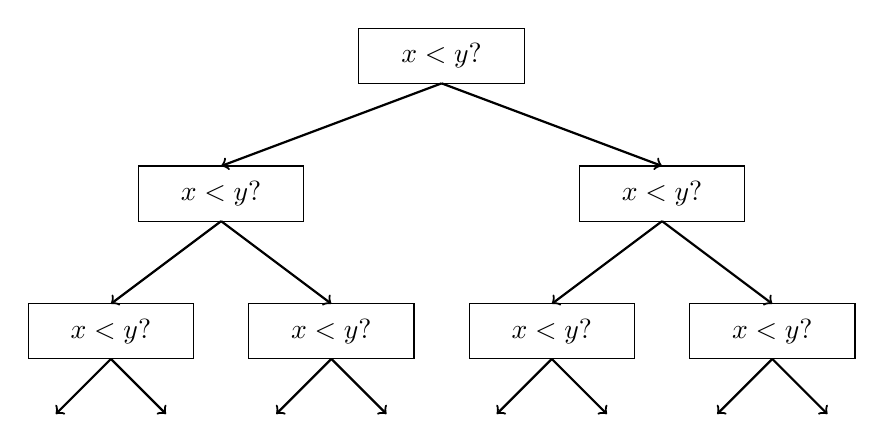
\begin{tikzpicture}[scale=0.7]
\draw (0,0) rectangle (3,1);
\node at (1.5,0.5) {$x < y?$};

\draw[thick,->] (1.5,0) -- (-2.5,-1.5);
\draw[thick,->] (1.5,0) -- (5.5,-1.5);

\draw (-4,-2.5) rectangle (-1,-1.5);
\draw (4,-2.5) rectangle (7,-1.5);
\node at (-2.5,-2) {$x < y?$};
\node at (5.5,-2) {$x < y?$};

\draw[thick,->] (-2.5,-2.5) -- (-4.5,-4);
\draw[thick,->] (-2.5,-2.5) -- (-0.5,-4);
\draw[thick,->] (5.5,-2.5) -- (3.5,-4);
\draw[thick,->] (5.5,-2.5) -- (7.5,-4);

\draw (-6,-5) rectangle (-3,-4);
\draw (-2,-5) rectangle (1,-4);
\draw (2,-5) rectangle (5,-4);
\draw (6,-5) rectangle (9,-4);
\node at (-4.5,-4.5) {$x < y?$};
\node at (-0.5,-4.5) {$x < y?$};
\node at (3.5,-4.5) {$x < y?$};
\node at (7.5,-4.5) {$x < y?$};

\draw[thick,->] (-4.5,-5) -- (-5.5,-6);
\draw[thick,->] (-4.5,-5) -- (-3.5,-6);
\draw[thick,->] (-0.5,-5) -- (0.5,-6);
\draw[thick,->] (-0.5,-5) -- (-1.5,-6);
\draw[thick,->] (3.5,-5) -- (2.5,-6);
\draw[thick,->] (3.5,-5) -- (4.5,-6);
\draw[thick,->] (7.5,-5) -- (6.5,-6);
\draw[thick,->] (7.5,-5) -- (8.5,-6);
\end{tikzpicture}
\end{center}

Qui ''$x<y?$'' significa che vengono confrontati 
due elementi qualsiasi $x$ e $y$.
Se $x<y$, il processo continua alla sinistra, 
altrimenti prosegue alla destra.
I risultati di questo processo sono i possibili
modi in dui un array può essere "disordinato", per un totale di $n!$ modi diversi,
cioè tutte le possibili permutazioni di $n$ elementi.
Per questa ragione l'altezza dell'albero 
deve essere almeno

\[ \log_2(n!) = \log_2(1)+\log_2(2)+\cdots+\log_2(n).\]

Il limite inferiore per questa somma può essere
stimato mantenendo solo gli ultimi $n/2$ elementi e
sostituendo ogni termine con $\log_2(n/2)$.
Il valore così ottenuto sarà minore di $log_2(n!)$, cioè 
\[ \log_2(n!) \ge (n/2) \cdot \log_2(n/2),\]
e quindi l'altezza dell'albero e il numero minimo 
di passaggi da effettuare nel caso pessimo 
sarà di tipo $O(n \log n)$.

\subsubsection{Counting sort}

\index{counting sort}

Il limite inferiore di $n \log n$ non riguarda gli algoritmi
di ordinamento che non usano il confronto tra due elementi,
ma utilizzano altre informazioni.
Un esempio in questo senso è l'algoritmo
\key{counting sort}, che ordina un array in
$O(n)$, nell'ipotesi che ogni elemento dell'array sia compreso tra
$0 \ldots c$ e $c=O(n)$.

Questo algoritmo crea un array di supporto, in cui gli indici
sono gli elementi dell'array da ordinare.
L'algoritmo itera attraverso tutto l'array da ordinare e,
per ogni elemento, incrementa il valore di un contatore
dell'array di supporto all'indirizzo corrispondente all'elemento.

Per esempio nell'array
\begin{center}
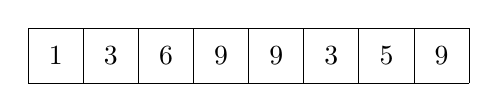
\begin{tikzpicture}[scale=0.7]
\draw (0,0) grid (8,1);
\node at (0.5,0.5) {$1$};
\node at (1.5,0.5) {$3$};
\node at (2.5,0.5) {$6$};
\node at (3.5,0.5) {$9$};
\node at (4.5,0.5) {$9$};
\node at (5.5,0.5) {$3$};
\node at (6.5,0.5) {$5$};
\node at (7.5,0.5) {$9$};
\end{tikzpicture}
\end{center}
genererà il seguente vettore di supporto:
\begin{center}
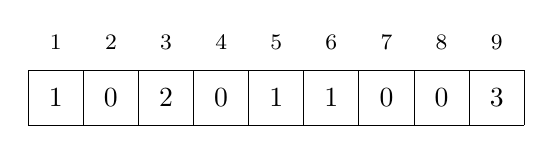
\begin{tikzpicture}[scale=0.7]
\draw (0,0) grid (9,1);
\node at (0.5,0.5) {$1$};
\node at (1.5,0.5) {$0$};
\node at (2.5,0.5) {$2$};
\node at (3.5,0.5) {$0$};
\node at (4.5,0.5) {$1$};
\node at (5.5,0.5) {$1$};
\node at (6.5,0.5) {$0$};
\node at (7.5,0.5) {$0$};
\node at (8.5,0.5) {$3$};

\footnotesize

\node at (0.5,1.5) {$1$};
\node at (1.5,1.5) {$2$};
\node at (2.5,1.5) {$3$};
\node at (3.5,1.5) {$4$};
\node at (4.5,1.5) {$5$};
\node at (5.5,1.5) {$6$};
\node at (6.5,1.5) {$7$};
\node at (7.5,1.5) {$8$};
\node at (8.5,1.5) {$9$};
\end{tikzpicture}
\end{center}

In questo esempio il valore alla posizione 3
nel vettore di supporto è 2,
perchè l'elemento di valore 3 compare due volte
nel vettore da ordinare.

La costruzione dell'array di supporto costa
$O(n)$ e fatto questo la creazione dell'array ordinato
prende solo $O(n)$, poichè per ogni elemento del vettore
di controllo vengono inseriti un certo numero di elementi 
corrispondenti all'indice, in base al valore dei contatori.
Quindi al complessità totale sarà ancora di tipo $O(n)$.

Il counting sort è molto efficiente, ma può essere usato
solo se la costante $c$ è sufficientemente piccola, in modo 
che i valori del vettore possano essere usati come indice
per l'array di supporto.

\section{Ordinamento in C++}

\index{ordinamento@\texttt{ordinamento}}

Durante una gara di informatica 
non è quasi mai una buona idea usare un 
algoritmo di ordinamento scritto da sè,
dal momento che tutti i linguaggi di programmazione
offrono delle ottime implementazioni
all'interno delle proprie librerie.
Per esempio, la libreria standard del C++
contiene la funzione \texttt{sort}
che può essere facilmente utilizzata
per ordinare vettori e altre strutture dati.

Usare una funzione di libreria comporta diversi vantaggi:
\begin{itemize}
\item si risparmia tempo perchè non c'è bisogno di scrivere
il codice che implementa l'ordinamento
\item l'implementazione di libreria è sicuramente
corretta e efficiente: è decisamente poco probabile
che la propria implementazione possa fare di meglio
\end{itemize}

In questa sezione si vedrà come utilizzare la
funzione \texttt{sort} del C++.
Il seguente codice ordina un vettore
in modo crescente:
\begin{lstlisting}
vector<int> v = {4,2,5,3,5,8,3};
sort(v.begin(),v.end());
\end{lstlisting}
Dopo l'ordinamento il contenuto del vettore sarà
$[2,3,3,4,5,5,8]$.
L'ordinamento di default è in senso crescente,
ma è possibile ordinare in senso decrescente così:
\begin{lstlisting}
sort(v.rbegin(),v.rend());
\end{lstlisting}
Oltre ai \emph{vector} di libreria del C++,
è possibile ordinare un normale array in questo modo:
\begin{lstlisting}
int n = 7; // array size
int a[] = {4,2,5,3,5,8,3};
sort(a,a+n);
\end{lstlisting}

Invece il seguente codice ordina la stringa \texttt{s}:
\begin{lstlisting}
string s = "monkey";
sort(s.begin(), s.end());
\end{lstlisting}
Ordinare una stringa significa ordinare i singoli
caratteri da cui è composta, quindi in questo esempio
''monkey'' diventerà ''ekmnoy''.

\subsubsection{Operatori di confronto}

\index{operatori di confronto}

La funzione \texttt{sort} richiede l'esistenza di un operatore 
di confronto che sia definito per i tipi che si intendono ordinare,
che verrà utilizzato nel momento in cui è necessario scoprire
l'ordine relativo di due elementi.

La maggior parte dei tipi di dato nativi del C++
hanno un operatore di confronto già definito e quindi
possono essere ordinati senza ulteriori specificazioni, 
come visto negli esempi precedenti, dove i numeri sono stati
ordinati in base al proprio valore e le lettere in ordine
alfabetico.

\index{pair@\texttt{pair}}

Le coppie (\texttt{pair}) sono ordinate in base al valore del primo elemento (\texttt{first}).
Però, se due coppie hanno lo stesso primo elemento, allora
l'ordinamento utilizzerà il secondo valore (\texttt{second}), per stabilire come ordinarli.
\begin{lstlisting}
vector<pair<int,int>> v;
v.push_back({1,5});
v.push_back({2,3});
v.push_back({1,2});
sort(v.begin(), v.end());
\end{lstlisting}
Dopo l'esecuzione, l'ordine delle coppie sarà
$(1,2)$, $(1,5)$ e $(2,3)$.

\index{tuple@\texttt{tuple}}

In un modo del tutto simile, le tuple (\texttt{tuple})
sono ordinate rispetto al loro primo elemento,
in caso di valori uguali si procede a confrontare il secondo elemento, ecc.
\footnote{Da notare che in alcuni vecchi compilatori è necessario utilizzare
la funzione \texttt{make\_tuple} per creare una tupla, al posto di usare la
notazione con le parentesi graffe (ad esempio \texttt{make\_tuple(2,1,4)} 
al posto di \texttt{\{2,1,4\}}).}:
\begin{lstlisting}
vector<tuple<int,int,int>> v;
v.push_back({2,1,4});
v.push_back({1,5,3});
v.push_back({2,1,3});
sort(v.begin(), v.end());
\end{lstlisting}
Dopo l'esecuzione le tuple saranno in questo ordine:
$(1,5,3)$, $(2,1,3)$ e $(2,1,4)$.

\subsubsection{Strutture definite dall'utente}

Le strutture definite dall'utente non hanno
un operatore di confronto se non viene creato appositamente.
L'operatore dovrebbe essere definito all'interno 
della struttura attraverso la ridefinizione dell'\texttt{operator<},
il cui unico parametro è un altro elemento dello stesso tipo.
L'operatore deve tornare \texttt{true}
se l'elemento è minore del parametro,
\texttt{false} altrimenti.

Per esempio, la seguente struttura \texttt{P}
contiene le coordinate x e y di un punto.
L'operatore di confronto è definito in modo che i 
punti verranno ordinati utilizzando la coordinata x,
e nel caso fossero uguali verrà utilizzata la coordinata y.

\begin{lstlisting}
struct P {
    int x, y;
    bool operator<(const P &p) {
        if (x != p.x) return x < p.x;
        else return y < p.y;
    }
};
\end{lstlisting}

\subsubsection{Comparison functions}

\index{comparison function}

It is also possible to give an external
\key{comparison function} to the \texttt{sort} function
as a callback function.
For example, the following comparison function \texttt{comp}
sorts strings primarily by length and secondarily
by alphabetical order:

\begin{lstlisting}
bool comp(string a, string b) {
    if (a.size() != b.size()) return a.size() < b.size();
    return a < b;
}
\end{lstlisting}
Now a vector of strings can be sorted as follows:
\begin{lstlisting}
sort(v.begin(), v.end(), comp);
\end{lstlisting}

\section{Binary search}

\index{binary search}

A general method for searching for an element
in an array is to use a \texttt{for} loop
that iterates through the elements of the array.
For example, the following code searches for
an element $x$ in an array:

\begin{lstlisting}
for (int i = 0; i < n; i++) {
    if (array[i] == x) {
        // x found at index i
    }
}
\end{lstlisting}

The time complexity of this approach is $O(n)$,
because in the worst case, it is necessary to check
all elements of the array.
If the order of the elements is arbitrary,
this is also the best possible approach, because
there is no additional information available where
in the array we should search for the element $x$.

However, if the array is \emph{sorted},
the situation is different.
In this case it is possible to perform the
search much faster, because the order of the
elements in the array guides the search.
The following \key{binary search} algorithm
efficiently searches for an element in a sorted array
in $O(\log n)$ time.

\subsubsection{Method 1}

The usual way to implement binary search
resembles looking for a word in a dictionary.
The search maintains an active region in the array,
which initially contains all array elements.
Then, a number of steps is performed,
each of which halves the size of the region.

At each step, the search checks the middle element
of the active region.
If the middle element is the target element,
the search terminates.
Otherwise, the search recursively continues
to the left or right half of the region,
depending on the value of the middle element.

The above idea can be implemented as follows:
\begin{lstlisting}
int a = 0, b = n-1;
while (a <= b) {
    int k = (a+b)/2;
    if (array[k] == x) {
        // x found at index k
    }
    if (array[k] > x) b = k-1;
    else a = k+1;
}
\end{lstlisting}

In this implementation, the active region is $a \ldots b$,
and initially the region is $0 \ldots n-1$.
The algorithm halves the size of the region at each step,
so the time complexity is $O(\log n)$.

\subsubsection{Method 2}

An alternative method to implement binary search
is based on an efficient way to iterate through
the elements of the array.
The idea is to make jumps and slow the speed
when we get closer to the target element.

The search goes through the array from left to
right, and the initial jump length is $n/2$.
At each step, the jump length will be halved:
first $n/4$, then $n/8$, $n/16$, etc., until
finally the length is 1.
After the jumps, either the target element has
been found or we know that it does not appear in the array.

The following code implements the above idea:
\begin{lstlisting}
int k = 0;
for (int b = n/2; b >= 1; b /= 2) {
    while (k+b < n && array[k+b] <= x) k += b;
}
if (array[k] == x) {
    // x found at index k
}
\end{lstlisting}

During the search, the variable $b$
contains the current jump length.
The time complexity of the algorithm is $O(\log n)$,
because the code in the \texttt{while} loop
is performed at most twice for each jump length.

\subsubsection{C++ functions}

The C++ standard library contains the following functions
that are based on binary search and work in logarithmic time:

\begin{itemize}
\item \texttt{lower\_bound} returns a pointer to the
first array element whose value is at least $x$.
\item \texttt{upper\_bound} returns a pointer to the
first array element whose value is larger than $x$.
\item \texttt{equal\_range} returns both above pointers.
\end{itemize}

The functions assume that the array is sorted.
If there is no such element, the pointer points to
the element after the last array element.
For example, the following code finds out whether
an array contains an element with value $x$:

\begin{lstlisting}
auto k = lower_bound(array,array+n,x)-array;
if (k < n && array[k] == x) {
    // x found at index k
}
\end{lstlisting}

Then, the following code counts the number of elements
whose value is $x$:

\begin{lstlisting}
auto a = lower_bound(array, array+n, x);
auto b = upper_bound(array, array+n, x);
cout << b-a << "\n";
\end{lstlisting}

Using \texttt{equal\_range}, the code becomes shorter:

\begin{lstlisting}
auto r = equal_range(array, array+n, x);
cout << r.second-r.first << "\n";
\end{lstlisting}

\subsubsection{Finding the smallest solution}

An important use for binary search is
to find the position where the value of a \emph{function} changes.
Suppose that we wish to find the smallest value $k$
that is a valid solution for a problem.
We are given a function $\texttt{ok}(x)$
that returns \texttt{true} if $x$ is a valid solution
and \texttt{false} otherwise.
In addition, we know that $\texttt{ok}(x)$ is \texttt{false}
when $x<k$ and \texttt{true} when $x \ge k$.
The situation looks as follows:

\begin{center}
\begin{tabular}{r|rrrrrrrr}
$x$ & 0 & 1 & $\cdots$ & $k-1$ & $k$ & $k+1$ & $\cdots$ \\
\hline
$\texttt{ok}(x)$ & \texttt{false} & \texttt{false}
& $\cdots$ & \texttt{false} & \texttt{true} & \texttt{true} & $\cdots$ \\
\end{tabular}
\end{center}

\noindent
Now, the value of $k$ can be found using binary search:

\begin{lstlisting}
int x = -1;
for (int b = z; b >= 1; b /= 2) {
    while (!ok(x+b)) x += b;
}
int k = x+1;
\end{lstlisting}

The search finds the largest value of $x$ for which
$\texttt{ok}(x)$ is \texttt{false}.
Thus, the next value $k=x+1$
is the smallest possible value for which
$\texttt{ok}(k)$ is \texttt{true}.
The initial jump length $z$ has to be
large enough, for example some value
for which we know beforehand that $\texttt{ok}(z)$ is \texttt{true}.

The algorithm calls the function \texttt{ok}
$O(\log z)$ times, so the total time complexity
depends on the function \texttt{ok}.
For example, if the function works in $O(n)$ time,
the total time complexity is $O(n \log z)$.

\subsubsection{Finding the maximum value}

Binary search can also be used to find
the maximum value for a function that is
first increasing and then decreasing.
Our task is to find a position $k$ such that

\begin{itemize}
\item
$f(x)<f(x+1)$ when $x<k$, and
\item
$f(x)>f(x+1)$ when $x \ge k$.
\end{itemize}

The idea is to use binary search
for finding the largest value of $x$
for which $f(x)<f(x+1)$.
This implies that $k=x+1$
because $f(x+1)>f(x+2)$.
The following code implements the search: 

\begin{lstlisting}
int x = -1;
for (int b = z; b >= 1; b /= 2) {
    while (f(x+b) < f(x+b+1)) x += b;
}
int k = x+1;
\end{lstlisting}

Note that unlike in the ordinary binary search,
here it is not allowed that consecutive values
of the function are equal.
In this case it would not be possible to know
how to continue the search.
